\documentclass[11pt, oneside]{article}   	% use "amsart" instead of "article" for AMSLaTeX format
\usepackage[margin=1in]{geometry}                		% See geometry.pdf to learn the layout options. There are lots.
\geometry{letterpaper}                   		% ... or a4paper or a5paper or ... 
%\geometry{landscape}                		% Activate for rotated page geometry
%\usepackage[parfill]{parskip}    		% Activate to begin paragraphs with an empty line rather than an indent
\usepackage{graphicx}				% Use pdf, png, jpg, or eps§ with pdflatex; use eps in DVI mode
								% TeX will automatically convert eps --> pdf in pdflatex		
\usepackage{amssymb}
\usepackage{awesomebox}
%SetFonts

%SetFonts

\usepackage{amsmath}
\DeclareMathOperator{\plainmod}{\text{ mod }}
\let\emptyset\varnothing

\newcommand{\reals}{\mathbb{R}}
\newcommand{\realsText}{$\mathbb{R}$}
\newcommand{\ints}{\mathbb{Z}}
\newcommand{\intsText}{$\mathbb{Z}$}

\title{Homework 7}
\author{Discrete Structures 2}
\date{due: 27 April 2023, 8:00am}							% Activate to display a given date or no date

\begin{document}
\maketitle
%\section{}
%\subsection{}

Your task for this homework will be to answer the following questions without using any calculating resources. 
Your responses should be submitted via blackboard by the due date above as a PDF (submissions in any other format will be returned to the user and a resubmissions will be requested). 
You are free to use whatever tools you would like to generate the response document: 
scanned hand-written paper, 
tablet generated hand-written, 
microsoft word (with this option, please use the equation editor to correctly format your responses), 
\LaTeX, etc.
Your TA, IA, and Instructor are available to help during their designated office hours or via email 
(note that emails sent during non-business hours may not be responded to until the next working day). 

%\importantbox{
%\textbf{Note:} all of these questions are on topics from chapters 5; thus you will only be proving by induction in this homework assignment. 
%}
\begin{enumerate}
\item Prove or disprove: in any tree with 3 or more nodes, there is a node of degree equal to 2.
\item Prove or disprove: in any rooted binary tree, there are an even number of leaves. (In a binary tree, all nodes have 0,1, or 2 children.)
\item Prove or disprove: if an undirected graph $G=\langle V,E\rangle$ has $|V|-1$ edges, then $G$ must be a forest.
\item Prove by induction that a complete binary tree of height $h$ contains precisely $2^{h+1}-1$ nodes.

\item Identify a minimum spanning trees in each of the following graphs. 
If a minimum spanning tree does not exist explain why under the graph.
\begin{center}
\hspace{-3em}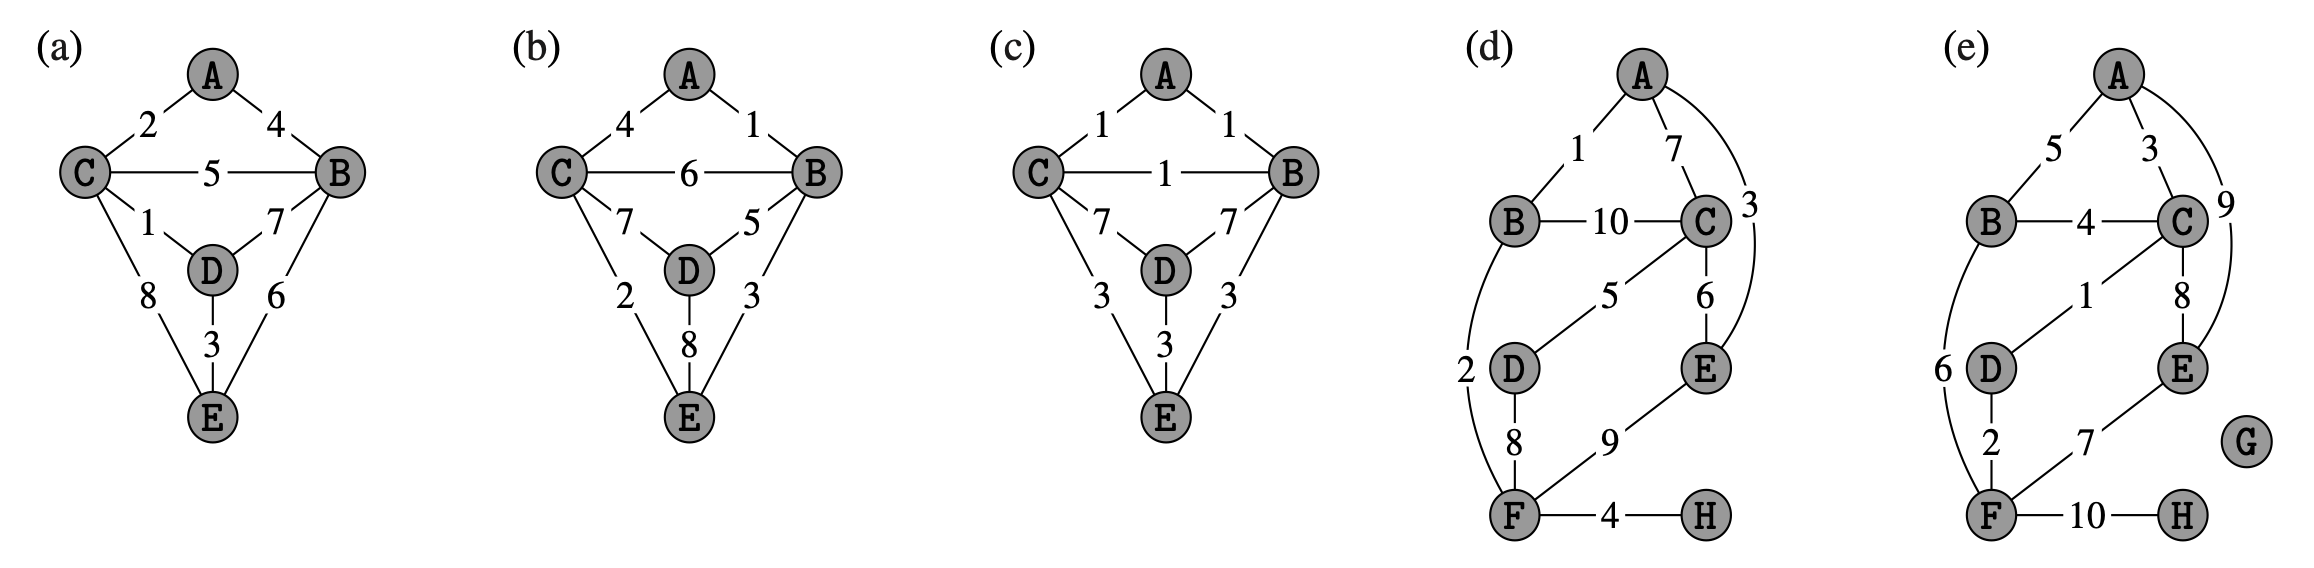
\includegraphics[width=\textwidth]{DS2-CH11-MST}
\end{center}


\item Prove or disprove: 
Let $G=\langle L\cup R,E\rangle$ be an undirected bipartite graph with $|L|=|R|$. 
Suppose every node in the graph (that is, all nodes in $L$ and $R$) has at least one neighbor. 
Then the graph is connected. 



\end{enumerate}
\end{document}